% chapters/seismo.tex
%
% Copyright 2022 Alexander Lyttle.
%
% This work may be distributed and/or modified under the conditions of the
% LaTeX Project Public License (LPPL) version 1.3 or later.
%
% The latest version of this license is in
% https://www.latex-project.org/lppl.txt and version 1.3 or later is part of
% all distributions of LaTeX version 2005/12/01 or later.
%
%
\chapter[Asteroseismology]{Asteroseismology of Solar-Like Oscillators}

Several decades ago, 5-minute oscillations of solar surface radial velocity were observed by \citet{Leighton.Noyes.ea1962}, leading to the inference of acoustic waves trapped beneath the solar photosphere \citep{Ulrich1970}. A further decade of study culminated in the measurement of individual oscillation modes in the Doppler shift \citep{Claverie.Isaak.ea1979} and total irradiance \citep{Woodard.Hudson1983a}. Initially thought to be short-lived irregularities on the surface, these modes were found to be compatible with stochastically excited standing waves penetrating deep into the Sun. Later, \citet{Deubner.Gough1984} introduced the word \emph{helioseismology} to describe the study of the solar interior using observation of these modes. Analogous to (geo)seismology, the characterisation and modelling of these oscillations lead to new insight into the solar interior, from measuring differential rotation \citep{Deubner.Ulrich.ea1979} to solving the mismatch between predicted and measured solar neutrino production \citep{Bahcall.Ulrich1988}.

% \begin{figure}[tbp]
%     \raggedleft
%     \begin{subfigure}[b]{0.25\linewidth}
%         
\includegraphics[width=\linewidth]{figures/spherical_harmonics/0_0.png}
%         \caption*{$l=0,\,m=0$}
%     \end{subfigure}%
%     \begin{subfigure}[b]{0.25\linewidth}
%         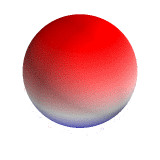
\includegraphics[width=\linewidth]{figures/spherical_harmonics/1_0.png}
%         \caption*{$l=1,\,m=0$}
%     \end{subfigure}%
%     \begin{subfigure}[b]{0.25\linewidth}
%         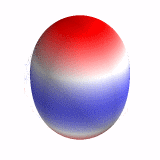
\includegraphics[width=\linewidth]{figures/spherical_harmonics/2_0.png}
%         \caption*{$l=2,\,m=0$}
%     \end{subfigure}%
%     \begin{subfigure}[b]{0.25\linewidth}
%         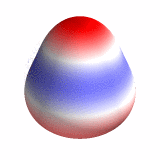
\includegraphics[width=\linewidth]{figures/spherical_harmonics/3_0.png}
%         \caption*{$l=3,\,m=0$}
%     \end{subfigure}%

%     \begin{subfigure}[b]{0.25\linewidth}
%         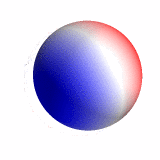
\includegraphics[width=\linewidth]{figures/spherical_harmonics/1_1.png}
%         \caption*{$l=1,\,m=1$}
%     \end{subfigure}%
%     \begin{subfigure}[b]{0.25\linewidth}
%         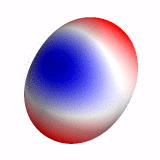
\includegraphics[width=\linewidth]{figures/spherical_harmonics/2_1.png}
%         \caption*{$l=2,\,m=1$}
%     \end{subfigure}%
%     \begin{subfigure}[b]{0.25\linewidth}
%         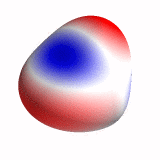
\includegraphics[width=\linewidth]{figures/spherical_harmonics/3_1.png}
%         \caption*{$l=3,\,m=1$}
%     \end{subfigure}%

%     \begin{subfigure}[b]{0.25\linewidth}
%         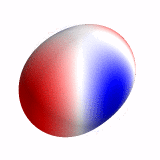
\includegraphics[width=\linewidth]{figures/spherical_harmonics/2_2.png}
%         \caption*{$l=2,\,m=2$}
%     \end{subfigure}%
%     \begin{subfigure}[b]{0.25\linewidth}
%         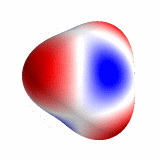
\includegraphics[width=\linewidth]{figures/spherical_harmonics/3_2.png}
%         \caption*{$l=3,\,m=2$}
%     \end{subfigure}%

%     \begin{subfigure}[b]{0.25\linewidth}
%         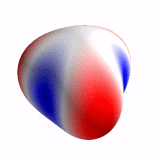
\includegraphics[width=\linewidth]{figures/spherical_harmonics/3_3.png}
%         \caption*{$l=3,\,m=3$}
%     \end{subfigure}
%     \caption{Spherical harmonic modes of oscillation for various combinations of angular degree ($l$) and azimuthal order ($m$).}
%     \label{fig:spherical-harmonics}
% \end{figure}

% Damped spherical harmonic oscillator \footnote{The spherical harmonic images were computed using code from \url{https://github.com/warrickball/spherical-harmonics}.}

% \begin{figure}[tb]
%     \centering
%     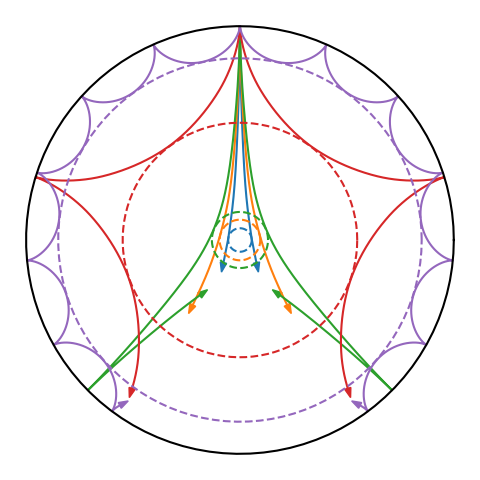
\includegraphics{figures/seismo-wavefronts.png}
%     \caption{The solid lines represent wavefronts of oscillation modes with different angular degree in a two-dimensional star. The dashed lines represent the turning-point of the wave. Lower angular degree modes propagate deeper into the star.}
%     \label{fig:seismo-wavefronts}
% \end{figure}

% The oscillations are stochastically excited at the stellar surface. Something about the wave fronts for each mode. How increasing angular degree corresponds to the angle of incidence at the stellar surface. Due to the monotonically increasing sound speed towards the centre of the star, the wavefront bends. We can see the turning points of the wavefronts in Figure \ref{fig:seismo-wavefronts}. Each modes propagation depth allows us to probe different regions of the star. In the case of the Sun, differential rotation. In other stars, low orders only visible.

Astronomers initially debated the mechanism driving solar oscillation modes attributed to standing pressure waves (so-called \emph{p-modes}). \citet{Goldreich.Keeley1977} suggested what became the prevailing theory, that the p-modes were stochastically excited by near-surface convection. Hence, we might expect solar-like oscillations to be present in other stars which have a convective envelope similar to the Sun. Shortly after, \citet{Christensen-Dalsgaard1984} introduced the term \emph{asteroseismology} --- the study of the internal structure of stars with many oscillation modes present. This differentiated it from studying the oscillations of classical variable stars where a small number of modes can only constrain the density of the star. Solar-like oscillations were first discovered in a few bright stars, notably Procyon and \(\alpha\) Cen A \citep{Gelly.Grec.ea1986}, with individual modes resolved by \citet{Martic.Schmitt.ea1999} and \citet{Bouchy.Carrier2001} respectively.

% in \(\varepsilon\) Eri \citep{Noyes.Baliunas.ea1984}

% \citet{Christensen-Dalsgaard1982} suggested that the limited precision of the radial velocity method made observing solar-like oscillations in many other stars difficult.
Instrumental and atmospheric noise largely limited the progress of asteroseismology to studies of small number of bright stars. With the advent of large-scale missions like \emph{CoRoT}, \emph{Kepler} and \emph{TESS}, we have gone from observing a handful to many thousands of solar-like oscillators. As such, asteroseismology has become a powerful tool for studying large populations of stars.

\begin{figure}[tb]
    \raggedleft
    \begin{subfigure}[b]{0.25\linewidth}
        
\includegraphics[width=\linewidth]{figures/spherical_harmonics/0_0.png}
        \caption*{$l=0$}
    \end{subfigure}%
    \begin{subfigure}[b]{0.25\linewidth}
        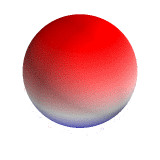
\includegraphics[width=\linewidth]{figures/spherical_harmonics/1_0.png}
        \caption*{$l=1$}
    \end{subfigure}%
    \begin{subfigure}[b]{0.25\linewidth}
        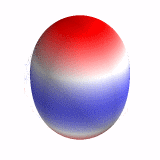
\includegraphics[width=\linewidth]{figures/spherical_harmonics/2_0.png}
        \caption*{$l=2$}
    \end{subfigure}%
    \begin{subfigure}[b]{0.25\linewidth}
        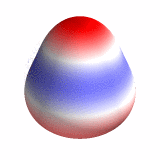
\includegraphics[width=\linewidth]{figures/spherical_harmonics/3_0.png}
        \caption*{$l=3$}
    \end{subfigure}%
    \caption{Exaggerated spherical harmonic oscillation modes for a few angular degrees ($l$). Red and blue represent represent regions extended radial outward and inward respectively. These regions oscillate between blue and red, with the white regions representing stationary nodes. \todo{Rotate these to show all of the nodes on the surface}.}
    \label{fig:spherical-harmonics}
\end{figure}

The p-mode oscillations are solutions to standing acoustic waves inside a star, governed by its interior physics and structure. Such spherical harmonic oscillators have unique solutions for integers (\(n, l\)). The radial order (\(n\)) is proportional to the number of radial nodes and the angular degree (\(l\)) is the number of nodes on a spherical shell of the star. We show a representation of this for the first four angular degrees in Figure \ref{fig:spherical-harmonics}. For each \(l\) there exists \(2l+1\) solutions with different azimuthal order (\(m\)) corresponding to the different orientations of the nodes over the spherical shell. In the case of a rotating or asymmetric star, the observed mode frequencies split for different \(m\) via the Doppler effect. Hereafter, we consider the case of a slowly rotating, spherically symmetric star, such that solutions of different \(m\) are approximately the same frequency.

Some stuff on how integrating brightness over the surface means the first few modes are observable.

P-modes in the solar-like oscillators are driven by near-surface convection. Typically, the timescale of this process drives high-order modes (\(n \sim 20\)). \citet{Tassoul1980} found that the mode frequencies could be approximated with the following expression by assuming the asymptotic limit where \(l/n \rightarrow 0\),
%
\begin{equation}
    \nu_{nl} \simeq \left(n + \frac{l}{2} + \varepsilon\right) \nu_0,
\end{equation}
%
where \(\varepsilon\) is some constant offset, \(\nu_0\) is the inverse of the acoustic diameter,
%
\begin{equation}
    \nu_0 = \left(2 \int_{0}^{R} \frac{\dd r}{c(r)}\right)^{-1},
\end{equation}
%
and \(c(r)\) is the sound speed as a function of radius.

The difference between consecutive modes of the same order \(\Delta\nu_{nl} = \nu_{nl} - \nu_{n-1\,l}\). In the same asymptotic limit, we expect \(\Delta\nu_{nl}\) to approximate \(\nu_0\). Therefore, we can reason that some measure of a global \(\Delta\nu\) (e.g. the average \(\langle\Delta\nu_{nl}\rangle\)) can give insight into the mean density of the star.

\begin{figure}[tb]
    \centering
    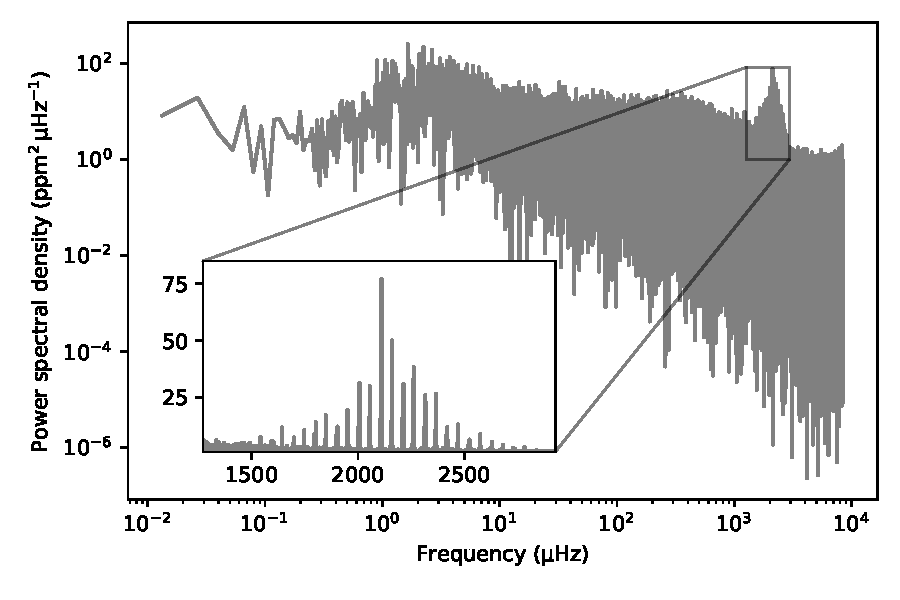
\includegraphics{figures/seismo-psd.pdf}
    \caption{The power spectral density of 16 Cyg A. The inset plot highlights the comb of peaks comprising a Gaussian-like hump in the larger plot.}
    \label{fig:seismo-psd}
\end{figure}

The 16 Cyg binary star system is home to two well-studied solar-like oscillators. As an example of what these observations look like, we will consider 16 Cyg A. Observed by \emph{Kepler} \todo{details like quarters}, the Kepler Asteroseismic Science Operations Center (KASOC\footnote{\url{https://kasoc.phys.au.dk}}) processed the light curve to extract the oscillation power spectrum. The details of their data reduction and processing can be found in \needcite. Briefly, creating a periodogram using the Lomb-Scargle method \citep{Lomb1976,Scargle1982}. We show the full power spectrum in Figure \ref{fig:seismo-psd}. We can see a clear Gaussian-like bump at around \SI{2000}{\micro\hertz}. Enlarging this, we see that it comprises a repeating patten of equally-spaced peaks.

\begin{figure}[tb]
    \centering
    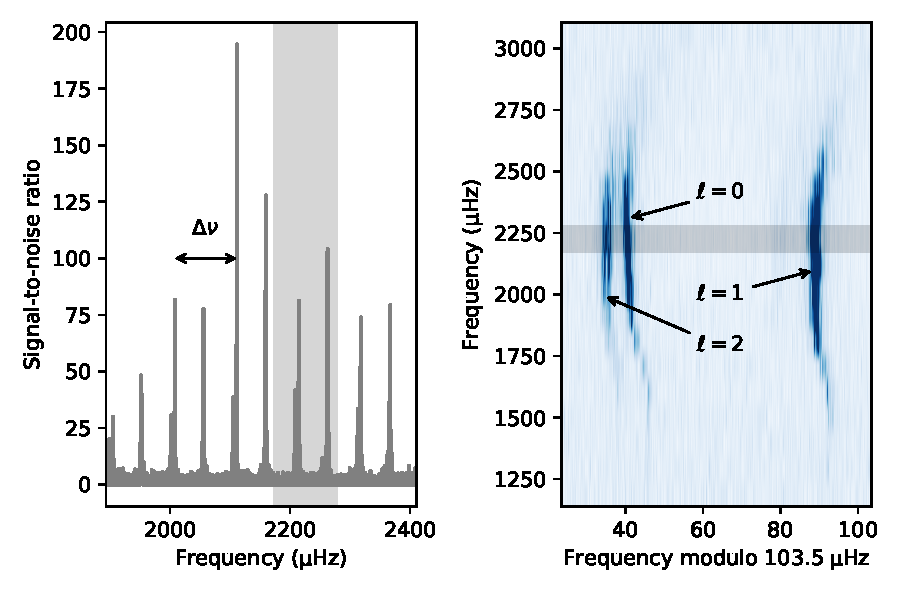
\includegraphics{figures/seismo-echelle.pdf}
    \caption{\emph{Left:} A section of the spectral signal-to-noise ratio (SNR) against frequency for 16 Cyg A. The large frequency spacing (\(\Delta\nu\)) between two radial modes is annotated with a double-headed arrow. The shaded region corresponds to a single row (also highlighted) in the echelle plot (\emph{right}). The echelle plot shows the spectral SNR such that a darker colour represents a higher SNR. Each row spans \SI{103.5}{\micro\hertz} and is stacked in order of frequency. The apparent ridges are labelled according to the angular degree (\(l\)) of the modes they represent.}
    \label{fig:seismo-echelle}
\end{figure}

The comb of peaks in the power spectrum corresponds to oscillation modes in the star. In Figure \ref{fig:seismo-echelle}, we show a small section of the power section with an estimate of the noise divided out. We see a regular repeating pattern, with similar modes repeated by approximately \(\Delta\nu\). If we wrap the spectrum by \(\Delta\nu\), we get the so-called echelle diagram. Ridges of high SNR correspond to modes of different angular degree. From the asymptotic expression, we expect modes of even angular degree grouped together, and likewise for odd angular degrees.

Looking at multiple stars we can see how the peak changes, this is frequency at maximum power. Scales with the acoustic cutoff frequency, so proportional to the surface gravity and effective temperature.

How can asteroseismology tell us about the star? Globally, we can use the scaling relations.

We can also use individual modes and compare with models. Worth noting the surface term here.
